%Caso de uso 2
\begin{UseCase} {CU1.1.2}{Agregar producto}{
	El empleado agregará los productos que el cliente desea comprar,saber el monto de cada medicamento,monto total y el número de productos agregados a la venta.
}

\UCitem{Versión}{1.0}
\UCccsection{Administración}
\UCccitem{Autor}{Lechuga Canales Héctor Jair}
\UCccitem{Evaluador}{Luis enrique Vázquez}
\UCccitem{Operación}{Ventas}
\UCccitem{Prioridad}{Alta}
\UCccitem{Complejidad}{Media}
\UCccitem{Volatilidad}{Baja}
\UCccitem{Madurez}{Alta}
\UCccitem{Estatus}{Edición}
\UCccitem{Fecha del último estatus}{04 de enero de 2022}

% Copie y pegue este bloque tantas veces como revisiones tenga el caso de uso.
% Esta sección la debe llenar solo el Revisor
% --------------------------------------------------------

% Revisión Versión 
% Anote la versión que se revisó
\UCccsection{Revisión Versión 0.1 }

% Fecha
% Anote la fecha en que se terminó la revisión
\UCccitem{Fecha}{03 de enero} 

% Evaluador
% Coloque el nombre completo de quien realizó la revisión
\UCccitem{Evaluador}{Luis enrique Vázquez}

% Resultado
% Coloque la palabra que mas se apegue al tipo de acción que el analista debe realizar
\UCccitem{Resultado}{redacción y ortografía}

% Observaciones
% Liste los cambios que debe realizar el Analista.
\UCccitem{Observaciones}{acentos y signos de puntuación}

% --------------------------------------------------------
	
\UCsection{Atributos}
	\UCitem{Actor(es)}
	{
		\cdtRef{Actor:RT}{Admimistrador de la farmacia}
	}
	\UCitem{Propósito}
	{
		Agregar productos al carrito de compras.
	}
	\UCitem{Entradas}
	{
		\UCli Código de barras
		\UCli Nombre
	}
	\UCitem{Salidas}
	{
		\UCli Código de barras 
		\UCli Descripción del producto
		\UCli Precio de venta
		\UCli Cantidad
	}

	\UCitem{Precondiciones}
	{
		\UCli El producto debe tener existencias. 
		\UCli El producto debe estar previamente ingresado en el sistema


	}
	\UCitem{Postcondiciones}
	{
		Ninguna
	}
	\UCitem{Reglas de negocio}
	{
		\cdtRef{RN-3}{Venta con receta médica.}
		\cdtRef{RN-7}{Cantidad de productos en carrito valida.}
	}
	\UCitem{Errores}
	{
		Ninguna
	}
	\UCitem{Tipo}{}
\end{UseCase}

%Trayectoria principal

\begin{UCtrayectoria}
		
	\UCpaso [\UCactor]Selecciona \cdtButton{Venta} en la interfaz del menú principal.Para visualizar la interfaz del menu principal visite a la página \pageref{UI: menu principal}
	\UCpaso [\UCsist]Muestra la interfaz carrito. Para visualizar la interfaz del carrito visite a la página \pageref{UI: carrito}
	\UCpaso [\UCactor]Escanea el código de barras de cada producto cuidando que se cumpla con la regla del negocio \cdtRef{RN-3}{Venta con receta médica}. \refTray{A}							
	\UCpaso [\UCsist]Obtiene los datos: Código de barras, nombre, descripción del producto, exixtencias y  p. venta de la BD. \refTray{B}
	\UCpaso [\UCsist]Muestra la lista de productos agregados con sus respectivos datos (Nombre, código de barras, descripción, cantidad agregada, precio de venta, subtotal). \refTray{C}
	\UCpaso [\UCsist]Muestra el total a pagar de la lista de productos agregados en un capo llamado “Precio total”.		

	
\end{UCtrayectoria}


% Trayectorias alternativas
% Trayectoria alternativa A

\begin{UCtrayectoriaA}{A}{El empleado no pudo escanear el código de barras o no tiene escaner}

	\UCpaso [\UCactor] Ingresa manualmente el código de los productos y seleciona el boton \cdtButton{Agregar} para agregar los artuculos al carrito.
	\UCpaso [\UCsist]Regresamos al 3 de la TP.
\end{UCtrayectoriaA}


%Trayectoria alternativa B

\begin{UCtrayectoriaA}{B}{No se puede conectar con la base de datos.}

	\UCpaso [\UCsist]Envía mensaje 1: "La base de datos no se encuentra disponible"
 	\UCpaso [\UCsist]Regresamos al paso 2 de la TP.

 \end{UCtrayectoriaA}

% Trayectoria alternativa C

\begin{UCtrayectoriaA}{C}{La cantidad de productos ingresada es mayor a la cantidad en existencia.}

	\UCpaso [\UCsist]Envía mensaje 2: "No hay suficientes productos en existencia"
	\UCpaso [\UCactor] Ajustar la cantidad del producto que no tiene suficiente existencia de acuerdo a la regla del negocio  \cdtRef{RN-7}{Cantidad de productos en carrito valida.}.
	\UCpaso [\UCsist]Regresamos al paso 5 de la TP.

\end{UCtrayectoriaA}

{
\begin{flushleft}
	% Clases
	\newpage
	\Large{Clases}\\
	\rule{14cm}{0.5pt}

	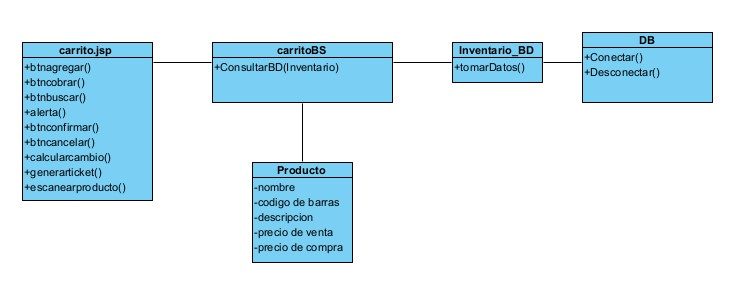
\includegraphics[width=14cm]{casouso/cu1.1.2/images/clases.jpg}\\	

	% Secuencia
	\newpage
	\Large{Secuencia}\\
	\rule{14cm}{0.5pt}

	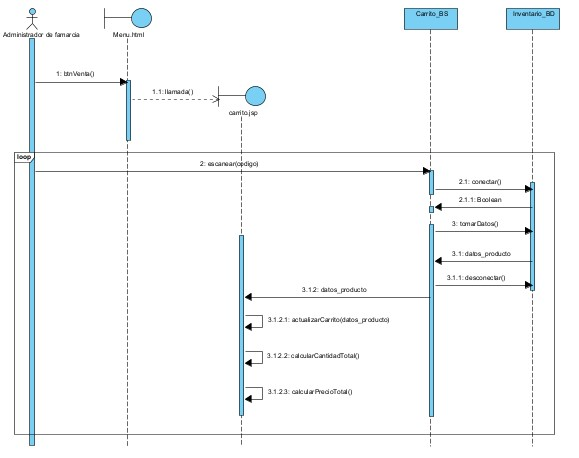
\includegraphics[width=14cm]{casouso/cu1.1.2/images/secuencia.jpg}\\	
	
\end{flushleft}
}